\section{Środowisko}\label{ux15brodowisko}

Dzięki nvidia-docker stosunkowo łatwo doprowadziłem do działania
obliczenia na GPU. Wygenerowałem w tym celu obraz z Dockerfile:

\begin{Shaded}
\begin{Highlighting}[]
\KeywordTok{FROM}\NormalTok{ tensorflow/tensorflow:latest-gpu-py3}

\KeywordTok{RUN}\NormalTok{ pip3 install --upgrade pip}

\KeywordTok{WORKDIR}\NormalTok{ /workdir}
\KeywordTok{COPY}\NormalTok{ requirements.txt /workdir/}

\KeywordTok{RUN}\NormalTok{ pip3 install -r <(grep -v tensorflow requirements.txt)}

\KeywordTok{COPY}\NormalTok{ . /workdir/}
\end{Highlighting}
\end{Shaded}

i uruchamiałem komendą

\begin{Shaded}
\begin{Highlighting}[]
\ExtensionTok{docker}\NormalTok{ run --runtime=nvidia -it -v }\VariableTok{$(}\BuiltInTok{pwd}\VariableTok{)}\NormalTok{:}\VariableTok{$(}\BuiltInTok{pwd}\VariableTok{)}\NormalTok{ --workdir }\VariableTok{$(}\BuiltInTok{pwd}\VariableTok{)}\NormalTok{ -u }\VariableTok{$(}\FunctionTok{id}\NormalTok{ -u}\VariableTok{)}\NormalTok{:}\VariableTok{$(}\FunctionTok{id}\NormalTok{ -g}\VariableTok{)}\NormalTok{ tfgpu:0.3O}
\end{Highlighting}
\end{Shaded}

\section{Zadanie 1}\label{zadanie-1}

Przygotowana funkcja generuje dla każdej warstwy podgląd 32 kanałów.
Kanały są równomiernie spośród wszystkich dostępnych, np. dla wartstwy o
960 kanałach pokazywany jest co trzydziesty.

Dla sieci ImageNet:

\begin{figure}
\centering
\includegraphics{./hw1/plot.png}
\caption{}
\end{figure}

\section{Zadanie 2}\label{zadanie-2}

Wszystkie ilustracje zostały przeskalowane do rozmiaru 224x224,
analogicznie jak to robi skrypt.

\subsection{Space shuttle}\label{space-shuttle}

Dokładność osiągnięta bez zaciemnienia: 86.09594\%

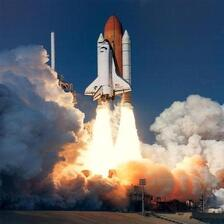
\includegraphics[width=2.33333in]{./hw2/shuttle.sq.jpg}
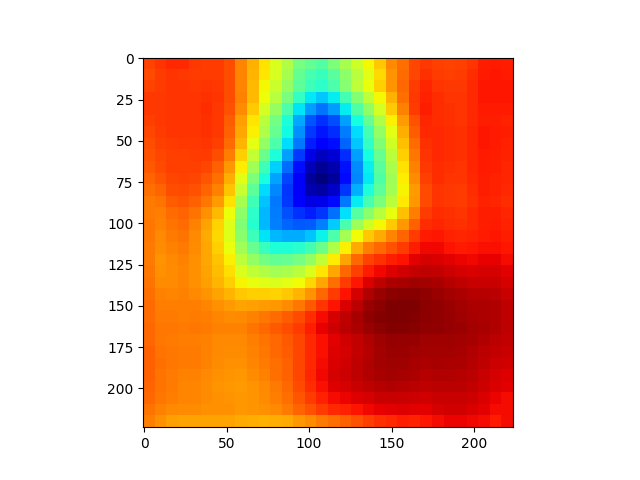
\includegraphics[width=3.64583in]{./hw2/shuttle.jpg.heatmap.png}

\subsection{Axolotl}\label{axolotl}

Dokładność osiągnięta bez zaciemnienia: 96.48967\%

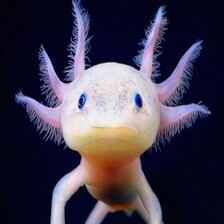
\includegraphics[width=2.33333in]{./hw2/out.jpg}
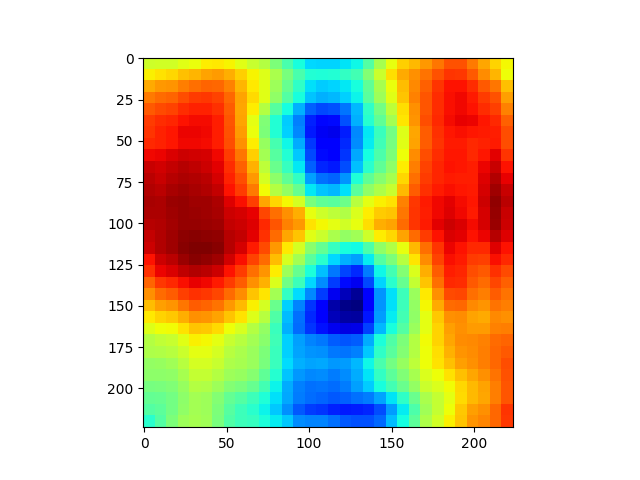
\includegraphics[width=3.64583in]{./hw2/axolotl.jpg.heatmap.png}
